\chapter{肾脏生理与渗透调节}\label{ch:b3:renal-osmoregulation}

你的肾脏每天滤过 180 升血浆——相当于每半小时便滤过一遍全身血液的体积——
其中除约 1.5 升外的全部都被回收，
同时清除尿素，并将盐、酸和水的含量调节到与机体需要量相差不超过 1\%，
葡萄糖则一克不漏地保留下来。
沙漠中的更格卢鼠从不饮水，
它依靠代谢干种子所产生的水生存，
并排出浓度为海水五倍的尿液。
海洋鱼类持续饮水，并经由鳃排出多余盐分；
淡水鱼从不饮水，却经由鳃主动摄入盐分。
它们所面临的问题本质相同：
在进食、饮水和呼吸扰动其成分的同时，维持细胞周围液体成分恒定，
并在排出含氮废物时不致丢失过多水分。
本章以哺乳动物肾脏作为典型实例，依次讨论
滤过、清除率的计算、使尿液浓缩的逆流机制，
以及设定这些“调节旋钮”的激素——
然后再介绍各类动物的各种渗透调节解决方案。

\section{问题}

\begin{definition}[渗透调节]\label{def:b3:renal-osmoregulation:problem}
\index{渗透浓度}\index{渗透压}\index{细胞外液}\index{渗透顺应者}\index{渗透调节者}
溶液的\emph{渗透浓度}是指其中溶解颗粒的总浓度
（以渗透摩尔每升计）；它决定\emph{渗透
压}，$\Pi = cRT$ 适用于稀溶液，它驱动水穿过
任何只允许水透过而不允许溶质透过的膜。哺乳动物的体液
渗透浓度约为 \qty{300}{mOsm/L}——\qty{40}{\%} 的体重位于细胞内，
\qty{20}{\%} 位于\emph{细胞外液}中，其四分之一为血浆——
若外界环境发生变化，细胞会在数秒内膨胀或收缩，
因为细胞膜可自由透水。
\emph{渗透顺应者}（大多数海洋无脊椎动物、鲨鱼）使体液的
渗透浓度与海水相同，只调节其成分；
\emph{渗透调节者}（脊椎动物、昆虫、
淡水动物）则使渗透浓度不随环境变化而保持恒定，
这需消耗与梯度成正比的能量。
第二项任务与第一项相关联，即处置蛋白质分解产生的含氮废物：
以\emph{氨}形式排入大量水中（鱼类）；
以\emph{尿素}形式排出，尿素可溶且无毒，但需借助水分运输（哺乳动物）；
或以\emph{尿酸}形式排出，它是一种几乎不含水的糊状物（鸟类、
爬行动物、昆虫）。
\end{definition}

\section{肾单位与滤过}

\begin{definition}[肾单位]\label{def:b3:renal-osmoregulation:nephron}
\index{肾单位}\index{肾小球}\index{近端小管}\index{髓袢}\index{集合管}
每个人肾脏约含 100 万个\emph{肾单位}。血液进入
一个\emph{肾\omterm{def:b3:sensory-systems:chemical}{小球}}，即位于肾小囊内的毛细血管丛，其
壁由有窗内皮、基膜以及
足细胞足突间的裂孔隔膜构成，允许水及所有
分子量低于约 \qty{60}{kDa} 的溶质通过，但截留蛋白质和细胞。滤液
依次流经\emph{近端小管}，该段重吸收三分之二的水和盐，
以及全部葡萄糖和氨基酸；随后
沿\emph{髓袢}下降并上升，髓袢伸入髓质，
并建立下一节所讨论的浓度梯度；随后经过
\emph{远端小管}，在此调节盐的含量；再进入
\emph{集合管}，其终尿含水量由
\omterm{prop:b3:renal-osmoregulation:countercurrent}{抗利尿激素}决定；集合管穿过髓质通向肾盂。离开
肾\omterm{def:b3:sensory-systems:chemical}{小球}的血液进入环绕小管的第二个毛细血管床，
并摄取小管所重吸收的物质。
\end{definition}

\begin{omfigure}
\begin{tikzpicture}[every node/.style={font=\scriptsize}, >=stealth]
  % cortex/medulla background
  \fill[omDef!6] (-0.5,0) rectangle (11.5,3.6); \fill[omProp!8] (-0.5,-3.4) rectangle (11.5,0);
  \node[right, gray] at (-0.4,3.4) {皮质}; \node[right, gray] at (-0.4,-3.2) {髓质};
  % glomerulus
  \draw[thick, omThm, fill=omThm!20] (0.8,2.6) circle (0.55); \node[below, align=center] at (0.25,2.0) {肾小球：\\滤过，\\\qty{180}{L/d}};
  % proximal tubule
  \draw[very thick, omDef] (1.35,2.6) .. controls (2.2,3.3) and (2.8,2.0) .. (3.2,2.6) .. controls (3.5,3.1) and (3.9,2.2) .. (4.2,2.6);
  \node[below, align=center] at (2.65,2.05) {近端小管：\\\qty{67}{\%} 的 Na$^{+}$ 和水，\\全部葡萄糖、氨基酸，\\HCO$_3^-$};
  % loop of Henle
  \draw[very thick, omDef] (4.2,2.6) -- (4.2,-2.8) arc[start angle=180, end angle=360, radius=0.4] -- (5.0,2.6);
  \node[left, align=right] at (4.1,-1.0) {降支：\\水分流出};
  \node[right, align=left] at (5.1,-1.6) {升支：\\泵出 NaCl，\\不透水};
  \node[right, align=left, omProp!80!black] at (5.1,-0.2) {\qty{25}{\%} 的 Na$^{+}$};
  % distal tubule
  \draw[very thick, omDef] (5.0,2.6) .. controls (5.4,3.2) and (6.0,2.0) .. (6.4,2.6) .. controls (6.8,3.1) .. (7.2,2.6);
  \node[above, align=center] at (6.0,3.1) {远端小管：Na$^{+}$（醛固酮调控），\\Ca$^{2+}$、K$^{+}$ 分泌};
  % collecting duct
  \draw[very thick, omMeth!70!black] (7.2,2.6) -- (7.8,2.6) -- (7.8,-3.2);
  \node[right, align=left] at (7.9,-1.2) {集合管：\\水（抗利尿激素、\\水通道蛋白-2），\\尿素、H$^{+}$；\\\qty{1.5}{L/d} 排出};
  \draw[->, thick, omMeth!70!black] (7.8,-3.2) -- (7.8,-3.6);
  % osmolarity scale on the right
  \foreach \y/\c in {2.6/300, 0.0/600, -1.4/900, -2.8/1200} { \node[left, omProp!80!black, font=\tiny] at (11.4,\y) {\c\ 毫渗透摩尔}; }
  \draw[->, omProp!80!black] (11.4,2.9) -- (11.4,-3.1); \node[above, omProp!80!black, font=\tiny, align=center] at (11.4,3.0) {间质 \\渗透浓度};
\end{tikzpicture}

{\small \omterm{def:b3:renal-osmoregulation:nephron}{肾单位}展开示意图。滤过发生于皮质；大量重吸收
发生于\omterm{def:b3:renal-osmoregulation:nephron}{近端小管}；\omterm{def:b3:renal-osmoregulation:nephron}{髓袢}深入髓质，
随深度增加，间质\omterm{def:b3:renal-osmoregulation:problem}{渗透浓度}愈高；\omterm{def:b3:renal-osmoregulation:nephron}{集合管}
回穿该梯度，并在\omterm{prop:b3:renal-osmoregulation:countercurrent}{抗利尿激素}允许时
释放水分。}
\end{omfigure}

\begin{theorem}[滤过与清除率]\label{thm:b3:renal-osmoregulation:clearance}
\index{斯塔林力}\index{肾小球滤过率}\index{清除率}\index{菊粉}\index{肌酐}
滤液穿过\omterm{def:b3:renal-osmoregulation:nephron}{肾小球}壁的速率由
\emph{\omterm{thm:b3:renal-osmoregulation:clearance}{斯塔林力}}决定：毛细血管的静水压
$P_{\text{GC}}$ 将液体推出，肾小囊腔内的静水压
$P_{\text{BS}}$ 与血浆蛋白的胶体\omterm{def:b3:renal-osmoregulation:problem}{渗透压}
$\pi_{\text{GC}}$ 则将其拉回，且
\[
\text{GFR} = K_{f}\,\bigl(P_{\text{GC}} - P_{\text{BS}} - \pi_{\text{GC}}\bigr)
\approx K_{f}\,(55 - 15 - 30)\ \unit{mmHg} = K_{f}\times \qty{10}{mmHg},
\]
即\emph{\omterm{thm:b3:renal-osmoregulation:clearance}{肾小球滤过率}}，成人中约为 \qty{125}{mL/min}。
对于任一物质 $x$，设其血浆浓度为 $P_{x}$，尿中
浓度为 $U_{x}$，尿流量为 $V$，其\emph{清除率}
\[
C_{x} = \frac{U_{x}\,V}{P_{x}}
\]
即单位时间内被清除 $x$ 的血浆体积。若 $x$ 可自由滤过，
既不被重吸收也不被分泌（\omterm{thm:b3:renal-osmoregulation:clearance}{菊粉}，肌酐与之近似），
则 $C_{x} = \text{GFR}$；若其被完全从
流经肾脏的血浆中清除（低剂量对氨基马尿酸），$C_{x}$
等于肾血浆流量；清除率低于 GFR 表示净重吸收，
高于则表示净分泌。滤过负荷 $\text{GFR}
\times P_{x}$ 减去排泄量 $U_{x}V$，即为被重吸收的量。
\end{theorem}
\begin{proof}
滤过即经多孔壁的超滤：流量
与其两侧的净压成正比，而净压为
向外的静水压减去向内的静水压与胶体\omterm{def:b3:renal-osmoregulation:problem}{渗透压}
（斯塔林），滤液的胶体\omterm{def:b3:renal-osmoregulation:problem}{渗透压}
可忽略，因其不含蛋白质。清除率：单位时间内
肾脏排出 $U_{x}V$ 量的 $x$；含有该量的血浆体积为
$U_{x}V/P_{x}$。对于只被滤过的物质，所排出的量
即为所滤过的量，$\text{GFR}\times P_{x} = U_{x}V$，
因此 $C_{x} = \text{GFR}$。对于被完全摄取的物质，流经肾脏的血浆中全部 $x$，
即 $\text{RPF}\times P_{x}$，被全部排出，
因此 $C_{x} = \text{RPF}$。由质量守恒可得被重吸收的量。
\end{proof}

\begin{example}[清除率的数值例子]\label{ex:b3:renal-osmoregulation:numbers}
\omterm{thm:b3:renal-osmoregulation:clearance}{菊粉}以血浆浓度 \qty{1}{mg/mL} 输注，尿中
浓度为 \qty{125}{mg/mL}，流速为 \qty{1}{mL/min}：$C = 125\times 1/1 =
\qty{125}{mL/min}$，即 GFR，折合 \qty{180}{L/d}。对氨基马尿酸
的清除率为 \qty{650}{mL/min}，即血浆流量；血细胞比容为 $0.45$，
则肾血流量为 \qty{1.2}{L/min}，为心输出量的五分之一，
而肾脏质量仅占体重的 \qty{0.5}{\%}，滤过分数为
$125/650 = 0.19$。尿素：血浆中 \qty{5}{mmol/L}，尿中 \qty{300}{mmol/L}
尿流速为 \qty{1}{mL/min}——清除率为 \qty{60}{mL/min}，为 GFR 的一半，故被滤过的尿素有一半
被重吸收。葡萄糖：正常
血浆水平下清除率为零，每日滤过的 \qty{180}{g} 葡萄糖
分子全部被回收。肌酐由肌肉以恒定速率生成，且仅被滤过，
是临床测定 GFR 的指标：GFR 减半时，
血浆肌酐即加倍，无需收集尿液。
\end{example}

\begin{method}[肾功能的测定]\label{met:b3:renal-osmoregulation:gfr}
\index{GFR 测定}
(1) 用于研究时，将\omterm{thm:b3:renal-osmoregulation:clearance}{菊粉}输注至稳定的血浆水平，
定时收集尿液，同时测定两者，并计算 $UV/P$。(2) 临床上，
测定血浆肌酐，并由此
用校正年龄、性别与体型的公式估算 GFR；该估计值
即慢性肾病分期所依据的标准（GFR
持续三个月低于 \qty{60}{mL/min}）。(3) 检验滤过\omterm{def:b3:innate-immunity:innate}{屏障}的选择性：
方法是测定尿中白蛋白，正常应低于
\qty{30}{mg/d}；超过则说明\omterm{def:b3:innate-immunity:innate}{屏障}渗漏，是
糖尿病肾\omterm{def:b3:dna-repair:lesions}{损伤}最早的征兆。(4) 检验浓缩能力：
夜间禁水后测定尿\omterm{def:b3:renal-osmoregulation:problem}{渗透浓度}，
正常应超过 \qty{800}{mOsm/L}；GFR 正常而浓缩功能不足，
提示\omterm{def:b3:renal-osmoregulation:nephron}{集合管}或\omterm{prop:b3:renal-osmoregulation:countercurrent}{抗利尿激素}有问题。
\end{method}

\begin{omfigure}
\begin{tikzpicture}
\begin{axis}[
  width=0.68\linewidth, height=5.6cm,
  axis x line=bottom, axis y line=left,
  xmin=0, xmax=800, ymin=0, ymax=700,
  xlabel={血浆葡萄糖 (mg/dL)}, ylabel={mg/min},
  xlabel style={font=\small, at={(axis description cs:0.5,-0.12)}, anchor=north}, ylabel style={font=\small},
  tick label style={font=\small}, xtick={0,100,200,300,400,600,800}, ytick={0,200,375,600},
  clip=false,
]
\addplot[very thick, omDef, domain=0:800, samples=2] {1.25*x};
\addplot[very thick, omMeth!70!black, domain=0:200, samples=2] {1.25*x};
\addplot[very thick, omMeth!70!black, smooth] coordinates {(200,250) (250,300) (300,340) (350,365) (400,375) (800,375)};
\addplot[very thick, omThm, domain=0:180, samples=2] {0};
\addplot[very thick, omThm, smooth] coordinates {(180,0) (250,12) (300,35) (350,72) (400,125) (800,625)};
\draw[dashed, gray] (axis cs:180,0) -- (axis cs:180,700); \node[font=\scriptsize, gray, anchor=north west] at (axis cs:185,560) {阈值};
\draw[dashed, gray] (axis cs:0,375) -- (axis cs:800,375);
\node[font=\scriptsize, omDef, anchor=south east] at (axis cs:480,620) {滤过量：GFR $\times$ P};
\node[font=\scriptsize, omMeth!70!black, anchor=south west, align=left] at (axis cs:660,395) {重吸收：\\$T_{m} = \qty{375}{mg/min}$};
\node[font=\scriptsize, omThm, anchor=north west] at (axis cs:520,300) {排泄};
\end{axis}
\end{tikzpicture}

{\small 葡萄糖滴定曲线。滤过负荷随血浆水平升高而增加，
\omterm{def:b3:renal-osmoregulation:nephron}{近端小管}的转运蛋白将其全部重吸收，
直至最大值 $T_{m}$；超过阈值时，约
为 \qty{180}{mg/dL}（\qty{10}{mmol/L}），葡萄糖溢入尿中 ---
即未经治疗的糖尿病患者尿中的糖。}
\end{omfigure}

\section{尿液的浓缩}

\begin{proposition}[逆流倍增]\label{prop:b3:renal-osmoregulation:countercurrent}
\index{逆流倍增}\index{单效应}\index{抗利尿激素}\index{水通道蛋白}\index{尿素再循环}
\omterm{def:b3:renal-osmoregulation:nephron}{髓袢}构建\omterm{def:b3:renal-osmoregulation:problem}{渗透浓度}梯度，由皮质处的 \qty{300}{mOsm/L}
升至髓质顶端的 \qty{1200}{mOsm/L}，
而任何细胞都无需对抗超过其中一部分的梯度。粗升支将其小管液中的 NaCl
泵入间质，且对水不通透，因此在每一水平，它使间质
比其自身管腔内液体约高 \qty{200}{mOsm/L}——
即\emph{\omterm{prop:b3:renal-osmoregulation:countercurrent}{单效应}}。降支对水通透，并与间质达到平衡，
因此向下流动的液体随下降而渐趋高渗，
到达弯曲处时已是浓缩液，升支随后从中泵出溶质；
向上流动的液体在每一水平都比间质更稀，
并以 \qty{100}{mOsm/L} 离开\omterm{def:b3:renal-osmoregulation:nephron}{髓袢}，为低渗液。
逆流使小的横向效应转化为大的纵向梯度：
弯曲处最咸的液体，是由本已高渗的液体
逐级形成的。\omterm{def:b3:renal-osmoregulation:nephron}{集合管}随后下行穿过
此梯度。无\emph{\omterm{prop:b3:renal-osmoregulation:countercurrent}{抗利尿激素}}时，
\omterm{def:b3:renal-osmoregulation:nephron}{集合管}管壁对水不通透，每小时可排出一升或更多稀释尿；
有之时，\emph{aquaporin-2} 通道插入管腔膜，
水顺梯度进入髓质，尿液\omterm{def:b3:renal-osmoregulation:problem}{渗透浓度}
达到髓质顶端的水平，即 \qty{1200}{mOsm/L}。
尿素自内层管道被重吸收，滞留于
髓质中，提供顶端\omterm{def:b3:renal-osmoregulation:problem}{渗透浓度}的一半；直小血管
本身呈逆流排列，
带走被重吸收的水，
且不
冲走梯度。
\end{proposition}

\begin{proof}[证据]
维尔茨、哈吉泰与库恩（1951）冷冻大鼠肾脏，并测定
皮质至乳头的切片中液体的熔点：
\omterm{def:b3:renal-osmoregulation:problem}{渗透浓度}随深度稳步升高，在
顶端达到尿液的数值——正是\omterm{prop:b3:renal-osmoregulation:countercurrent}{逆流倍增}理论（库恩，
一位物理化学家，1942 年）所要求的梯度。小管微穿刺
（戈特沙尔克，1959 年）随后发现，\omterm{def:b3:renal-osmoregulation:nephron}{髓袢}弯曲处的液体为高渗，
离开升支的液体为低渗，
\omterm{def:b3:renal-osmoregulation:nephron}{集合管}内液体在每一水平都与间质相同，此时
存在\omterm{prop:b3:renal-osmoregulation:countercurrent}{抗利尿激素}。生活于沙漠的啮齿类，\omterm{def:b3:renal-osmoregulation:nephron}{髓袢}最长者
梯度最陡，尿液也最为浓缩。
\end{proof}

\begin{omfigure}
\begin{tikzpicture}[every node/.style={font=\scriptsize}, >=stealth]
  % loop
  \draw[very thick, omDef] (0,3.2) -- (0,-0.4) arc[start angle=180, end angle=360, radius=0.7] -- (1.4,3.2);
  \draw[very thick, omDef] (0.35,3.2) -- (0.35,-0.4) arc[start angle=180, end angle=360, radius=0.35] -- (1.05,3.2);
  % interstitial osmolarity bands
  \foreach \y/\c/\col in {2.8/300/10, 2.0/500/25, 1.2/700/40, 0.4/900/55, -0.4/1100/70, -1.0/1200/80} { \fill[omProp!\col, opacity=0.5] (-2.2,\y-0.4) rectangle (-0.2,\y+0.4); \node[left, font=\tiny] at (-2.25,\y) {\c}; }
  \node[left, align=right, font=\tiny] at (-2.25,3.35) {间质 \\(mOsm/L)};
  % arrows: water out of descending, NaCl out of ascending
  \foreach \y in {2.4,1.6,0.8,0.0} { \draw[->, thick, omDef!70!black] (0.15,\y) -- (-0.4,\y); }
  \node[left, omDef!70!black, font=\tiny] at (-0.45,2.4) {H$_2$O};
  \foreach \y in {2.4,1.6,0.8,0.0} { \draw[->, thick, omThm] (1.25,\y) -- (1.9,\y); }
  \node[right, omThm, font=\tiny] at (1.5,2.85) {NaCl 泵出};
  % fluid osmolarity labels inside limbs
  \node[above] at (0.17,3.25) {\qty{300}{} 入}; \node[above] at (1.22,3.25) {\qty{100}{} 出};
  \node[font=\tiny] at (0.7,-1.35) {弯曲处 1200};
  \node[below, align=center] at (0.2,-1.7) {降支：水流出，\\液体浓缩；升支：\\盐流出，液体稀释};
  % collecting duct
  \draw[very thick, omMeth!70!black] (4.2,3.2) -- (4.2,-1.4); \node[above, align=center] at (4.2,3.25) {集合管};
  \foreach \y in {2.4,1.6,0.8,0.0,-0.8} { \draw[->, thick, omMeth!70!black] (4.1,\y) -- (3.5,\y); }
  \node[right, align=left, font=\tiny] at (4.3,1.2) {有抗利尿激素：\\aquaporin-2 插入，\\水沿梯度流出};
  \node[below, align=center] at (4.2,-1.5) {尿液达到 \\\qty{1200}{mOsm/L}};
  % single effect note
  \node[right, align=left] at (6.4,2.6) {单效应：升支使间质在每一水平 \\保持比其自身液体高 $\sim\qty{200}{mOsm/L}$；\\逆流使效应逐级叠加，\\形成自皮质至乳头达 \qty{900}{mOsm/L} 的梯度};
\end{tikzpicture}

{\small \omterm{prop:b3:renal-osmoregulation:countercurrent}{逆流倍增}器。从升支泵出的盐
使间质呈高渗；降支中被吸出的水在
液体到达泵之前使其浓缩；反向流动
使微小的横向差异逐级叠加为
四倍梯度，\omterm{def:b3:renal-osmoregulation:nephron}{集合管}利用该梯度在
\omterm{prop:b3:renal-osmoregulation:countercurrent}{抗利尿激素}使其对水开放时浓缩尿液。}
\end{omfigure}

\begin{proposition}[水的算术]\label{prop:b3:renal-osmoregulation:water}
\index{必需失水}\index{自由水清除率}
机体若须每日排出溶质负荷 $S$（约
\qty{600}{mOsm}，主要为尿素与盐）时，尿\omterm{def:b3:renal-osmoregulation:problem}{渗透浓度}至多为
$U_{\max}$，则所需最小尿量为 $V_{\min} = S/U_{\max}$：对
人而言，$600/1200 = \qty{0.5}{L}$ 每天，即\emph{\omterm{prop:b3:renal-osmoregulation:water}{必需失水}}
量，另加肺和皮肤散失的约 \qty{0.9}{L}。饮用
海水（约 \qty{1000}{mOsm/L}，几乎全为盐）每升水含
\qty{1000}{mOsm} 的盐，须排出；以
$U_{\max}$ 计，排出这些盐需 $1000/1200 = \qty{0.83}{L}$ 尿液，但
盐还需连同尿素负荷一并排出，净得水量
接近零甚至为负：饮用海水的遇难水手
脱水比不饮用者更快。\emph{\omterm{prop:b3:renal-osmoregulation:water}{自由水
清除率}}，$V - U_{\text{osm}}V/P_{\text{osm}}$，是
肾在单位时间内向体内加入或从体内移除的无溶质水的体积，
在水负荷（稀释尿）时为正，
脱水时为负。
\end{proposition}
\begin{proof}
溶质仅经尿液排出（不计汗液），浓度至多
$U_{\max}$，故 $S = U V \le U_{\max}V$，得 $V \ge S/U_{\max}$。对海
水而言：每升带入 \qty{1000}{mOsm}；以
\qty{1200}{mOsm/L} 排出需 \qty{0.83}{L}，剩余 \qty{0.17}{L}，
未计当日自身代谢产生的 \qty{600}{mOsm} 溶质，其
排出还要消耗它。\omterm{prop:b3:renal-osmoregulation:water}{自由水清除率}：体积为 $V$ 的尿液
\omterm{def:b3:renal-osmoregulation:problem}{渗透浓度}为 $U_{\text{osm}}$，所含溶质为 $U_{\text{osm}}V$，
在血浆\omterm{def:b3:renal-osmoregulation:problem}{渗透浓度}下将占据体积 $U_{\text{osm}}V/P_{\text{osm}}$；其
余下的体积即为超出此量的水，从体内被清除。
\end{proof}

\begin{omfigure}
\begin{tikzpicture}
\begin{axis}[
  width=0.66\linewidth, height=5.4cm,
  axis x line=bottom, axis y line=left,
  xmin=0, xmax=1300, ymin=0, ymax=12,
  xlabel={尿渗透浓度 (mOsm/L)}, ylabel={尿量 （L/天）},
  xlabel style={font=\small, at={(axis description cs:0.5,-0.12)}, anchor=north}, ylabel style={font=\small},
  tick label style={font=\small}, xtick={50,300,600,1200}, ytick={0.5,2,6,12},
  clip=false,
]
\addplot[very thick, omDef, domain=50:1300, samples=100] {600/x};
\draw[dashed, gray] (axis cs:300,0) -- (axis cs:300,2); \draw[dashed, gray] (axis cs:1200,0) -- (axis cs:1200,0.5);
  \node[font=\scriptsize, omDef, anchor=south west] at (axis cs:350,3.5) {$V = S/U$ 其中 $S = \qty{600}{mOsm/d}$};
  \node[font=\scriptsize, anchor=west, align=left] at (axis cs:1210,1.7) {最大浓缩：\\\qty{0.5}{L}};
  \node[font=\scriptsize, anchor=south west] at (axis cs:60,9) {最大稀释（\qty{50}{mOsm/L}）：\qty{12}{L}};
\end{axis}
\end{tikzpicture}

{\small 运载一天溶质所需的尿量，随其
浓度变化。从肾能产生的最稀释尿到
最浓缩尿，尿量相差二十四倍；
\omterm{prop:b3:renal-osmoregulation:countercurrent}{抗利尿激素}决定所处的位置。}
\end{omfigure}

\section{调节}

\begin{definition}[调节机制]\label{def:b3:renal-osmoregulation:controls}
\index{肾素–血管紧张素–醛固酮系统}\index{醛固酮}\index{心房利钠肽}\index{渗透压感受器}\index{管球反馈}
两个变量分别受调节：\omterm{def:b3:renal-osmoregulation:problem}{细胞外液}的\emph{体积}，
取决于机体保留多少钠。另一个是其
\emph{\omterm{def:b3:renal-osmoregulation:problem}{渗透浓度}}，取决于水。体积方面：
球旁器的细胞，位于远端小管
与自身\omterm{def:b3:renal-osmoregulation:nephron}{肾小球}的小动脉相接处，在动脉压或小管盐量降低时释放\emph{肾素}；
肾素从血浆蛋白上切下血管紧张素 I，
转换酶生成\emph{血管紧张素 II}，
使小动脉收缩、刺激口渴，并
促使肾上腺皮质释放\emph{醛固酮}，数小时内使
远端小管和\omterm{def:b3:renal-osmoregulation:nephron}{集合管}重吸收钠（经由通道 ENaC）并分泌钾。
被牵张的心房释放\emph{利钠肽}，作用相反。\omterm{def:b3:renal-osmoregulation:problem}{渗透浓度}方面：
\omterm{def:b3:nervous-systems:plan}{下丘脑}的\emph{\omterm{def:b3:renal-osmoregulation:problem}{渗透压}感受器}感知到 \qty{1}{\%} 的升高，并
在数分钟内促使垂体后叶释放\omterm{prop:b3:renal-osmoregulation:countercurrent}{抗利尿激素}，
并引起口渴；下降则使其停止。肾脏也能自我调节：
\emph{管球反馈}使远端盐输送过高的\omterm{def:b3:renal-osmoregulation:nephron}{肾单位}的小动脉收缩，
以使每个\omterm{def:b3:renal-osmoregulation:nephron}{肾单位}的滤过量不超过其小管所能处理的范围。
酸碱平衡方面：\omterm{def:b3:renal-osmoregulation:nephron}{近端小管}回收滤过的碳酸氢根，
\omterm{def:b3:renal-osmoregulation:nephron}{集合管}逆千倍梯度分泌质子，
质子以磷酸盐缓冲后排出，
最主要的是以由谷氨酰胺生成的铵形式
排出 ---
这是机体排除
富含蛋白质饮食所产之酸的途径。
\end{definition}

\begin{omfigure}
\begin{tikzpicture}[every node/.style={font=\scriptsize}, >=stealth]
  \node[draw, thick, rounded corners, fill=omThm!20, align=center] (low) at (0,0) {动脉压低 \\或小管 NaCl 浓度低};
  \node[draw, thick, rounded corners, fill=omDef!20, align=center] (ren) at (3.6,0) {球旁器 \\细胞释放肾素};
  \node[draw, thick, rounded corners, fill=omDef!20, align=center] (ang) at (7.4,0) {血管紧张素 I $\to$ II\\（转换酶）};
  \node[draw, thick, rounded corners, fill=omMeth!25, align=center] (ald) at (11.0,1.2) {醛固酮：\\Na$^{+}$ 潴留，K$^{+}$ 流失};
  \node[draw, thick, rounded corners, fill=omMeth!25, align=center] (vc) at (11.0,-0.3) {小动脉收缩};
  \node[draw, thick, rounded corners, fill=omMeth!25, align=center] (th) at (11.0,-1.8) {口渴，抗利尿激素};
  \draw[->, thick] (low) -- (ren); \draw[->, thick] (ren) -- (ang);
  \draw[->, thick] (ang) -- (ald.west); \draw[->, thick] (ang) -- (vc.west); \draw[->, thick] (ang) -- (th.west);
  \node[draw, thick, rounded corners, fill=omProp!25, align=center] (res) at (6.8,-2.6) {体积与压力恢复};
  \draw[->, thick] (ald.east) -- ++(0.4,0) |- (res.east); \draw[thick] (vc.east) -- ++(0.4,0); \draw[thick] (th.east) -- ++(0.4,0);
  \draw[-|, thick, omThm] (res.south) -- ++(0,-0.6) -| (low.south) node[pos=0.3, below, font=\tiny] {负反馈};
  \node[draw, thick, rounded corners, fill=gray!15, align=center, font=\tiny] (anp) at (2.4,-2.6) {牵张心房：\\利钠肽，作用相反};
  \draw[-|, thick, gray!60!black] (anp.east) -- (res.west);
\end{tikzpicture}

{\small 肾素–血管紧张素–\omterm{def:b3:renal-osmoregulation:controls}{醛固酮}环路，是机体
钠及由此决定的\omterm{def:b3:renal-osmoregulation:problem}{细胞外液}体积的慢速调节器。血管紧张素 II
同时作用于血管、肾上腺、脑和肾脏；利钠
肽来自被牵张的心脏，与之拮抗。}
\end{omfigure}

\begin{example}[两天]\label{ex:b3:renal-osmoregulation:two-days}
无水一天：血浆\omterm{def:b3:renal-osmoregulation:problem}{渗透浓度}由 $290$ 升至
约 \qty{295}{mOsm/L}，\omterm{prop:b3:renal-osmoregulation:countercurrent}{抗利尿激素}在数分钟内升高，\omterm{def:b3:renal-osmoregulation:nephron}{集合管}
对水开放，尿液浓缩至 \qty{1200}{mOsm/L}，
尿量降至半升；此人口渴；失去的水量
主要来自细胞，细胞中的水随细胞外的盐分而流出。
一次饮下一升水：\omterm{def:b3:renal-osmoregulation:problem}{渗透浓度}下降 \qty{1}{\%}，
\omterm{prop:b3:renal-osmoregulation:countercurrent}{抗利尿激素}在二十分钟内降至零，\omterm{def:b3:renal-osmoregulation:nephron}{集合管}关闭，
接下来两小时内，肾脏排出一升尿液，\omterm{def:b3:renal-osmoregulation:problem}{渗透浓度}为
\qty{50}{mOsm/L}。一次失血一升：血压下降，
肾素和\omterm{prop:b3:renal-osmoregulation:countercurrent}{抗利尿激素}均升高（容量压过\omterm{def:b3:renal-osmoregulation:problem}{渗透浓度}），
小动脉收缩，钠与水被保留，一天之内
血浆容量得以补充——液体取自组织间隙，
再经饮水补足。尿崩症，即\omterm{prop:b3:renal-osmoregulation:countercurrent}{抗利尿激素}或其
受体缺失，每日产生 \qty{15}{L} 稀释尿液，并伴有与之相称的
口渴；肾衰竭，即滤过功能丧失，机体
须每周三次借助机器滤过，经由一层膜
其清除率仅为两个肾脏的一部分。
\end{example}

\begin{omfigure}
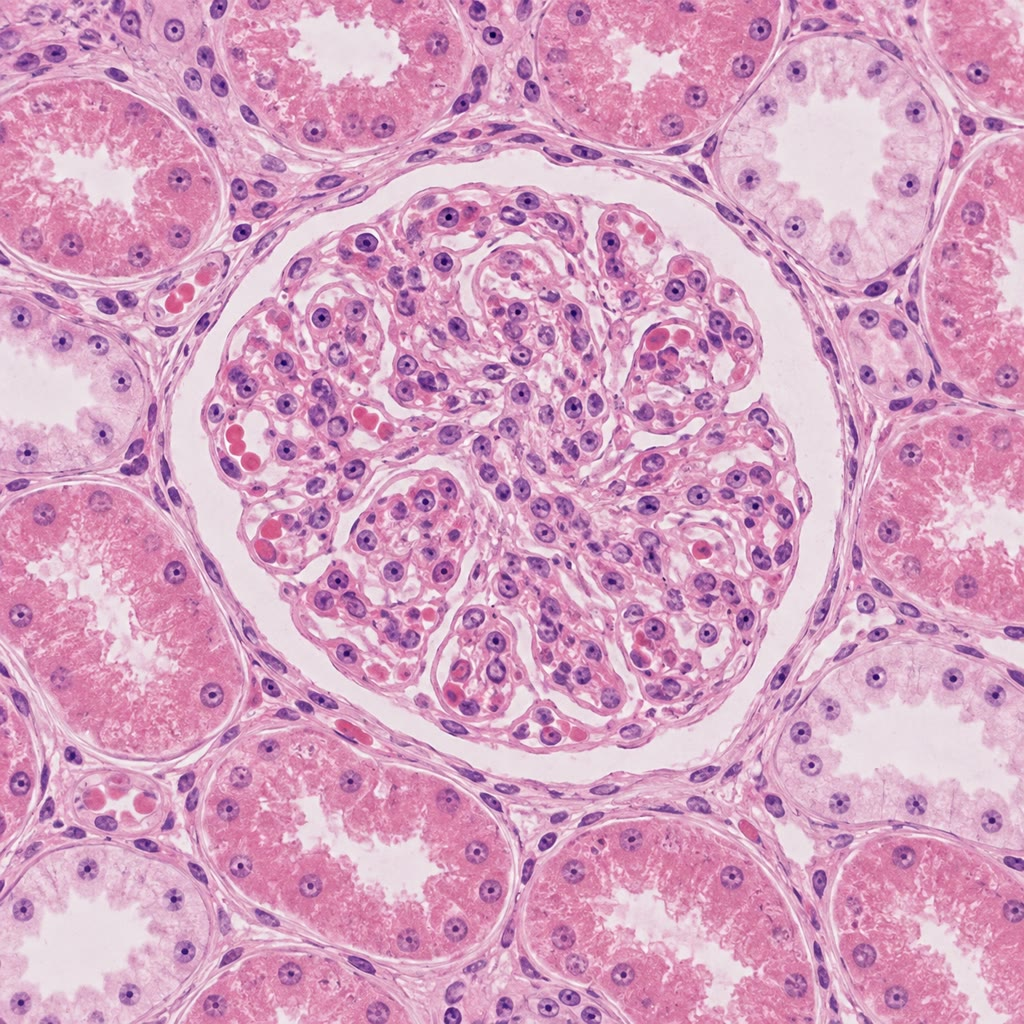
\includegraphics[width=0.46\linewidth]{images/book5/ai/b5-20-kidney-section.jpg}\hspace{0.04\linewidth}
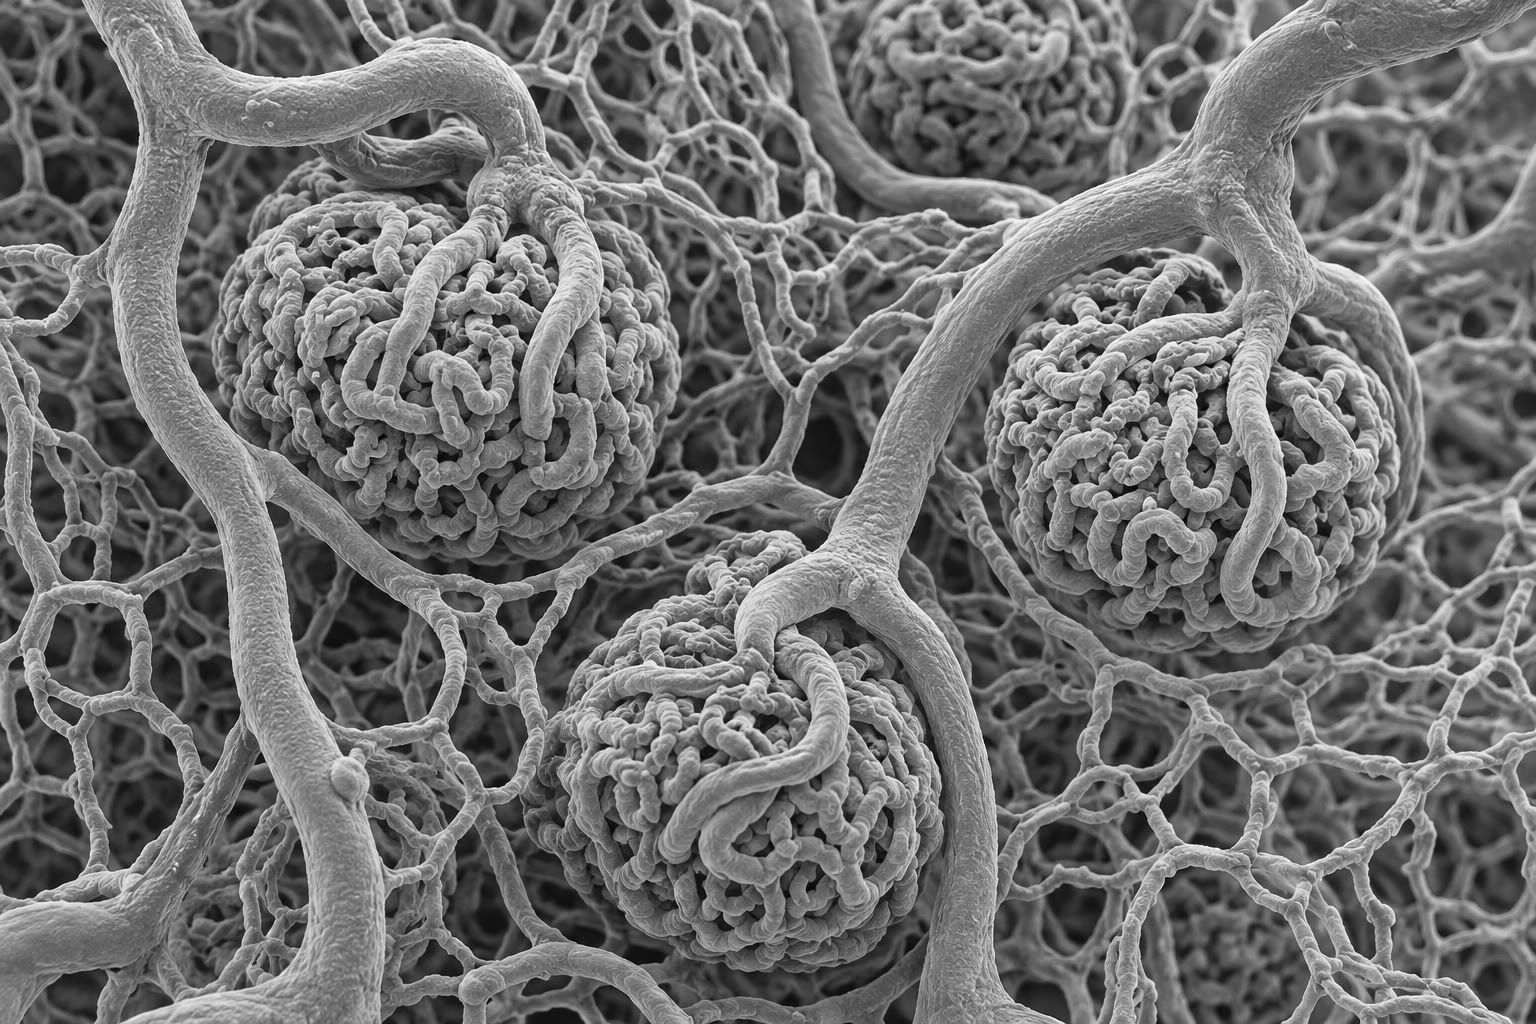
\includegraphics[width=0.46\linewidth]{images/book5/ai/b5-20-nephron-cast.jpg}

{\small 左：肾皮质切片——\omterm{def:b3:renal-osmoregulation:nephron}{肾小球}及其肾小囊，
位于近端与远端小管的断面之间。右：皮质的血管
铸型，每团“线球”即一个\omterm{def:b3:renal-osmoregulation:nephron}{肾小球}及其入球
与出球小动脉，穿插于管周毛细血管之间。}
\end{omfigure}

\section{其他动物，其他溶液}

\begin{definition}[动物间的渗透调节]\label{def:b3:renal-osmoregulation:comparative}
\index{马氏管}\index{盐腺}\index{泌氯细胞}\index{代谢水}\index{相对髓质厚度}
淡水鱼生活在\omterm{def:b3:renal-osmoregulation:problem}{渗透浓度}仅为其血液十分之一的介质中：
水经鳃大量涌入，盐分外漏，它们
排出大量稀释尿液，并经鳃的
\emph{泌氯细胞}主动吸收盐分，从不饮水。海洋硬骨鱼的血液
\omterm{def:b3:renal-osmoregulation:problem}{渗透浓度}为海水的三分之一，经鳃失水，饮入海水，
并经同一批泌氯细胞（功能逆转）将盐分泵出，
尿量极少；鲨鱼则使血液与海水等渗，
借保留尿素（并以氧化三甲胺
稳定蛋白质以抵御尿素），并经直肠腺排出多余盐分。
海鸟与海洋爬行动物在眼上方具有\emph{盐腺}，
可分泌盐度为海水两倍的浓盐水，使
信天翁得以饮用海水。昆虫则经
\emph{马氏管}过滤，由主动分泌钾驱动，而非血压，
并在直肠中重吸收水分，程度之高，
以至沙漠甲虫的粪便干燥。哺乳动物中，
浓缩能力随\omterm{def:b3:renal-osmoregulation:nephron}{髓袢}长度相对于
肾脏大小（即\emph{相对髓质厚度}）而定：河狸
可达 \qty{500}{mOsm/L}，人类 \num{1200}，骆驼 \num{3000}，
袋鼠鼠 \num{5500}——使其能依靠食物氧化时释放的\emph{代谢
水}，每克淀粉氧化可得约 \qty{0.6}{g} 水，
并借一只鼻子，通过逆流冷却，从每次呼出的
气息中回收水分。
\end{definition}

\begin{omfigure}
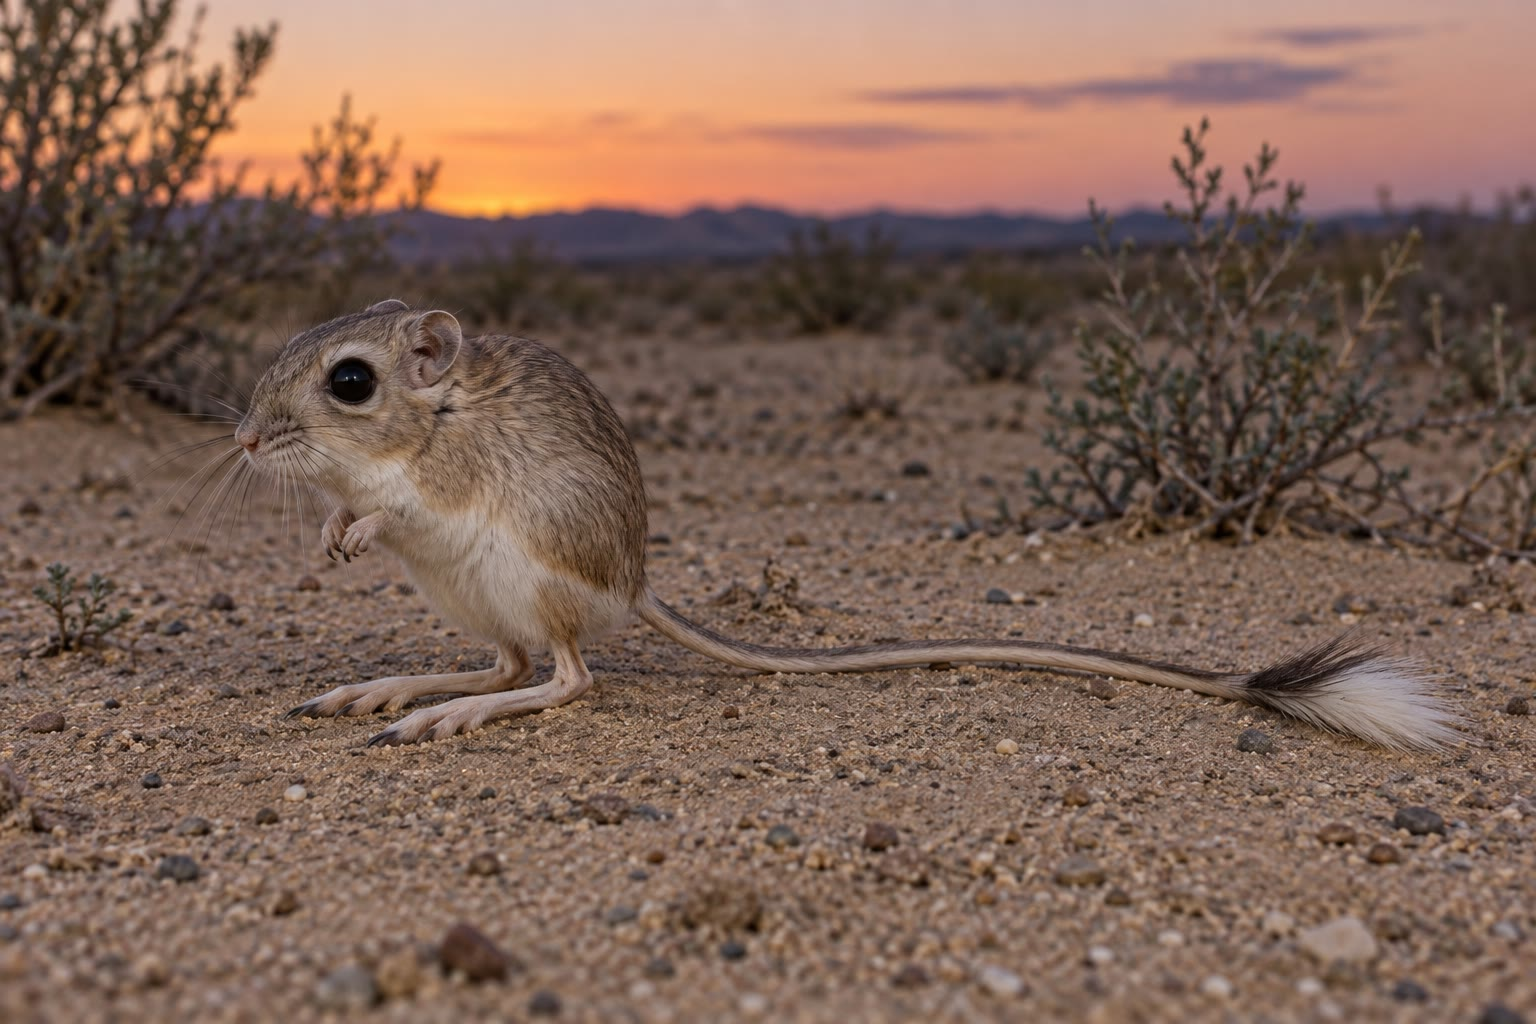
\includegraphics[width=0.56\linewidth]{images/book5/ai/b5-20-kangaroo-rat.jpg}

{\small 袋鼠鼠，从不饮水：\omterm{def:b3:renal-osmoregulation:nephron}{髓袢}很长，尿液
浓度为海水的五倍，凉爽的鼻子使每次呼出的
水汽凝结，食物氧化生成的水足以满足
其全部需要。}
\end{omfigure}

\begin{remark}[作为设计问题的肾脏]\label{rem:b3:renal-osmoregulation:design}
哺乳动物肾脏每天滤过的血浆量为血浆容量的四十倍，
却几乎全部重吸收回来：这是一种奢侈的设计，其要点在于
滤过一切再选择性重吸收，比
选择性地分泌每一种可能出现的废物更为简单。其代价是
静息代谢的 \qty{7}{\%}，用于泵回钠，其脆弱之处
在于精细的滤器，它在
高压与高血糖下缓慢失效。其巧妙之处在于逆流
环路，这一装置也见于深海鱼的鳔、
涉禽的腿以及沙漠啮齿动物的鼻子中，借此，一个小而
可承受的局部差异被叠加为一个大的差异——其思想
在各种情形中都是同一个：梯度可以由流动建立。
\end{remark}

\section{练习}

\begin{exercise}[$\star$]\label{exo:b3:renal-osmoregulation:1}
依次写出\omterm{def:b3:renal-osmoregulation:nephron}{肾单位}各段的名称，并简述各段
的一项功能。
\end{exercise}

\begin{exercise}[$\star$]\label{exo:b3:renal-osmoregulation:2}
定义清除率。某物质的血浆浓度为
\qty{2}{mg/mL}，尿中浓度为 \qty{100}{mg/mL}，尿流量为
\qty{1.5}{mL/min}。计算其清除率，并判断该物质
是被重吸收、被分泌还是两者皆非（已知 GFR 为 \qty{120}{mL/min}）。
\end{exercise}

\begin{exercise}[$\star$]\label{exo:b3:renal-osmoregulation:3}
为什么淡水鱼从不饮水而海水鱼
需不断饮水？两类鱼的鳃各起什么作用？
\end{exercise}

\begin{exercise}[$\star$]\label{exo:b3:renal-osmoregulation:4}
\omterm{def:b3:renal-osmoregulation:nephron}{髓袢}的\omterm{prop:b3:renal-osmoregulation:countercurrent}{单效应}是什么？哪一支产生该效应，
且两支对水的通透性为何必须不同？
\end{exercise}

\begin{exercise}[$\star\star$]\label{exo:b3:renal-osmoregulation:5}
\omterm{def:b3:renal-osmoregulation:nephron}{肾小球}毛细血管压为 \qty{60}{mmHg}，鲍曼囊
压为 \qty{18}{mmHg}，血浆胶体\omterm{def:b3:renal-osmoregulation:problem}{渗透压}在入球端为 \qty{28}{mmHg}，
在出球端升至 \qty{35}{mmHg}。计算两端的净
滤过压，并说明滤过为何可能在毛细血管
末端之前停止。这对血浆流量对 GFR 的影响
意味着什么？
\end{exercise}

\begin{exercise}[$\star\star$]\label{exo:b3:renal-osmoregulation:6}
患者的肌酐清除率为 \qty{40}{mL/min}，血浆钠为
\qty{140}{mmol/L}，尿钠为 \qty{70}{mmol/L}，尿流量为
\qty{1}{mL/min}。计算钠的滤过负荷、排泄量、
重吸收比例及钠的清除率。
\end{exercise}

\begin{exercise}[$\star\star$]\label{exo:b3:renal-osmoregulation:7}
某人每日饮食产生 \qty{900}{mOsm} 溶质，尿液最高可
浓缩至 \qty{1200}{mOsm/L}。最少尿量为多少？若肾病
使最高浓缩能力降至 \qty{400}{mOsm/L}，则此人需饮水多少
才能维持水平衡（设不显性失水为 \qty{0.9}{L}）？
\end{exercise}

\begin{exercise}[$\star\star$]\label{exo:b3:renal-osmoregulation:8}
预测下列情况下的尿量、尿\omterm{def:b3:renal-osmoregulation:problem}{渗透浓度}、血浆钠浓度及口渴状态：
(a) 尿崩症，(b) \omterm{def:b3:cancer-biology:hallmarks}{肿瘤}引起的\omterm{prop:b3:renal-osmoregulation:countercurrent}{抗利尿激素}
（血管加压素）分泌不当，(c) \omterm{def:b3:renal-osmoregulation:controls}{醛固酮}过多，(d) 一周无
盐饮食。
\end{exercise}

\begin{exercise}[$\star\star$]\label{exo:b3:renal-osmoregulation:9}
计算尿\omterm{def:b3:renal-osmoregulation:problem}{渗透浓度}为 \qty{100}{mOsm/L}、尿流量为
\qty{6}{mL/min} 时的\omterm{prop:b3:renal-osmoregulation:water}{自由水清除率}，以及尿\omterm{def:b3:renal-osmoregulation:problem}{渗透浓度}为 \qty{1000}{mOsm/L}
、尿流量为 \qty{0.6}{mL/min} 时的\omterm{prop:b3:renal-osmoregulation:water}{自由水清除率}（血浆\omterm{def:b3:renal-osmoregulation:problem}{渗透浓度}为 \qty{300}{mOsm/L}），并分别解释其含义。
\end{exercise}

\begin{exercise}[$\star\star\star$]\label{exo:b3:renal-osmoregulation:10}
将\omterm{def:b3:renal-osmoregulation:nephron}{髓袢}建模为 $n$ 个阶段，每一阶段上升支液体的
\omterm{def:b3:renal-osmoregulation:problem}{渗透浓度}比间质低 \qty{200}{mOsm/L}，降支液体与间质相等，
液体以 \qty{300}{mOsm/L} 进入。论证弯曲处的稳态\omterm{def:b3:renal-osmoregulation:problem}{渗透浓度}
可接近 $300 +
200n$，因而梯度受限于\omterm{def:b3:renal-osmoregulation:nephron}{髓袢}长度及
泵的\omterm{prop:b3:renal-osmoregulation:countercurrent}{单效应}，并从物理上说明何者决定 $n$。
\end{exercise}

\begin{exercise}[$\star\star\star$]\label{exo:b3:renal-osmoregulation:11}
一只更格卢鼠每日食用 \qty{5}{g} 干种子，其中淀粉占 \qty{80}{\%}，
经氧化生成 CO$_{2}$ 和水（每克淀粉生成 \qty{0.6}{g} 水）。
它每日须排出 \qty{3}{mOsm} 溶质，尿\omterm{def:b3:renal-osmoregulation:problem}{渗透浓度}为 \qty{5500}{mOsm/L}，
并每日经鼻腔蒸发失去 \qty{1.5}{g} 水，其鼻腔
可回收呼气中 \qty{70}{\%} 的水分。请配平其水分收支，
并说明它在不饮水时能否存活。
\end{exercise}

\begin{exercise}[$\star\star\star$]\label{exo:b3:renal-osmoregulation:12}
透析时血液沿膜的一侧流动，透析液沿另一侧
逆向流动。试说明逆流的清除效果为何优于并流，
并估算一台透析机的清除率，该机
以 \qty{70}{\%} 的效率从 \qty{300}{mL/min} 血液中清除尿素，
并比较：若该机每周运行三次、每次四小时，
其清除量与双肾一周的清除量相比如何。
\end{exercise}

\section{问题：一日十八桶}

\begin{problem}[{周末问题——追踪一日滤液自肾小球至膀胱的过程：
斯塔林压力、四种物质的清除率、
葡萄糖阈值、从最大稀释到海水的水分收支，
以及一种沙漠啮齿动物的水平衡，最后求出
肾小球滤过率、必需尿量，以及一升海水能
获得的净水量}]
\label{pb:b3:renal-osmoregulation:1}
数据：$K_{f} = \qty{12.5}{mL/min/mmHg}$；$P_{\text{GC}} = \qty{55}{mmHg}$，
$P_{\text{BS}} = \qty{15}{mmHg}$, $\pi_{\text{GC}} = \qty{30}{mmHg}$.
血浆：\omterm{thm:b3:renal-osmoregulation:clearance}{菊粉} \qty{0.5}{mg/mL}、肌酐 \qty{0.01}{mg/mL}、尿素
\qty{5}{mmol/L}、葡萄糖 \qty{5}{mmol/L}、对氨基马尿酸
\qty{0.02}{mg/mL}、Na$^{+}$ \qty{140}{mmol/L}、\omterm{def:b3:renal-osmoregulation:problem}{渗透浓度}
\qty{290}{mOsm/L}。尿流量 \qty{1}{mL/min}：\omterm{thm:b3:renal-osmoregulation:clearance}{菊粉} \qty{62.5}{mg/mL}，
肌酐 \qty{1.3}{mg/mL}、尿素 \qty{250}{mmol/L}、葡萄糖 $0$，
对氨基马尿酸 \qty{13}{mg/mL}、Na$^{+}$ \qty{100}{mmol/L}，
\omterm{def:b3:renal-osmoregulation:problem}{渗透浓度} \qty{600}{mOsm/L}。血细胞比容 $0.45$。葡萄糖 $T_{m} =
\qty{375}{mg/min}$（\qty{2.1}{mmol/min}）。每日溶质 \qty{600}{mOsm}；
$U_{\max} = \qty{1200}{mOsm/L}$，$U_{\min} = \qty{50}{mOsm/L}$；
不显性失水 \qty{0.9}{L/d}；海水 \qty{1000}{mOsm/L}。

\medskip
\noindent\textbf{第一部分——滤过器。}
\begin{enumerate}
  \item 计算净滤过压和 GFR。
  \item 将 GFR 换算为每日升数。
        血浆容量（\qty{3}{L}）被滤过多少次？
  \item 计算\omterm{thm:b3:renal-osmoregulation:clearance}{菊粉}清除率，并与 GFR 比较。
        计算肌酐清除率；为何它略大？
  \item 计算对氨基马尿酸清除率（即肾血浆流量）、
        肾血流量及滤过分数。
  \item 出球小动脉收缩，使 $P_{\text{GC}}$ 升至
        \qty{60}{mmHg}。新的 GFR 为多少？为何阻断血管紧张素 II 的药物
        在健康肾脏中仅使 GFR 略有降低，却能保护
        糖尿病患者的肾脏？
  \item 尿中出现蛋白质，速率为 \qty{3}{g/d}。滤过器的哪一层
        已失效？若此情况持续，血浆胶体\omterm{def:b3:renal-osmoregulation:problem}{渗透压}
        及组织会发生怎样的变化？
\end{enumerate}

\medskip
\noindent\textbf{第二部分——处理过程。}
\begin{enumerate}[resume]
  \item 尿素：滤过负荷、排泄量、重吸收比例，
        以及清除率。
  \item 钠：每日滤过负荷（以摩尔和克计）、排泄量，
        以及重吸收比例。若全部不被重吸收，
        一日将损失多少千克食盐？
  \item 葡萄糖：以 mmol/min 及每日克数计的滤过负荷，是否有
        葡萄糖被排出？血浆葡萄糖为多少时，滤过负荷
        达到 $T_{m}$（阈值）？
  \item 某糖尿病患者血浆葡萄糖为 \qty{20}{mmol/L}，其每分钟及每日排出的
        葡萄糖（以克计）各为多少，以及额外尿量（按当时浓度，
        每 \qty{300}{mOsm} 葡萄糖需 \qty{1}{L} 尿液携带）。
        试解释未经治疗的糖尿病为何引起口渴及体重
        下降。
  \item 重吸收钠每 3 个 Na$^{+}$ 消耗 1 个 ATP。肾脏每日
        为钠消耗多少摩尔 ATP，合多少千焦
        （\qty{50}{kJ/mol}）？与静息时的
        \qty{7}{MJ/d}.
  \item 试说明肾脏为何对各种废物采用滤过和重吸收，而不是
        分泌。试从小管需要识别什么的角度
        加以说明。
\end{enumerate}

\medskip
\noindent\textbf{第三部分——水。}
\begin{enumerate}[resume]
  \item 由数据求\omterm{def:b3:renal-osmoregulation:problem}{渗透浓度}清除率 $U_{\text{osm}}V/P_{\text{osm}}$，
        以及\omterm{prop:b3:renal-osmoregulation:water}{自由水清除率}。判断该个体是在保存水分，
        还是在排出水分？
  \item 求每日溶质所需的最小尿量；求最大尿量（在
        $U_{\min}$ 下）；求最小尿量下的每日总需水量，
        计入不显性失水。
  \item 饮用一升海水。需要多少尿液才能
        以 $U_{\max}$ 排出其中的盐分，净水分增益是多少？
        计入当日自身溶质之前是多少？计入之后呢？
  \item \omterm{prop:b3:renal-osmoregulation:countercurrent}{抗利尿激素}缺失（尿崩症），尿液量维持在
        $U_{\min}$。求同样溶质下的每日尿量，以及
        每日为维持平衡须饮用的水量。
  \item 啤酒的\omterm{def:b3:renal-osmoregulation:problem}{渗透浓度}为 \qty{20}{mOsm/L}。在 $U_{\min}$ 下，肾脏已
        无法再排出水分，此时每日最多可饮用多少？
        （超过 $U_{\min}$ 下溶质所能携带之量的水分
        会蓄积。）
  \item 一夜未饮水后，血浆\omterm{def:b3:renal-osmoregulation:problem}{渗透浓度}为
        \qty{298}{mOsm/L}。其升高了百分之几？\omterm{def:b3:nervous-systems:plan}{下丘脑}做了什么？
        若全身水量为
        \qty{42}{L}、溶质不变，估算水分缺乏量。
  \item 解释马拉松选手饮用 \qty{6}{L} 水、同时出汗失盐时，
        为何会出现危险的低血浆钠，
        以及肾脏需要做什么才能防止这种情况。
\end{enumerate}

\medskip
\noindent\textbf{第四部分——沙漠。}
\begin{enumerate}[resume]
  \item 更格卢鼠每日排出 \qty{3}{mOsm} 溶质，尿液浓度为 \qty{5500}{mOsm/L}。
        尿量是多少？将其与人类肾脏在自身最大浓缩能力下
        排出同样溶质所需的尿量相比较。
  \item 其食物每日产生 \qty{2.4}{g} \omterm{def:b3:renal-osmoregulation:comparative}{代谢水}，每日经呼吸损失 \qty{1.6}{g}，
        经粪便损失 \qty{0.3}{g}。
        结合第 20 题中的尿量，核算其水分收支平衡。
  \item 骆驼可将尿液浓缩至 \qty{3000}{mOsm/L}，并能耐受损失 \qty{25}{\%} 的体水。
        对于体重 \qty{500}{kg}、含水量为 \qty{65}{\%} 的骆驼，
        它最多可损失多少水？以每日损失 \qty{5}{L/d} 计，
        这些水可维持多少天？
  \item 一只海鸟每日摄入 \qty{200}{g} 鱼，并饮用 \qty{100}{mL} 海水，
        同时摄入 \qty{150}{mmol} 氯化钠。其\omterm{def:b3:renal-osmoregulation:comparative}{盐腺}以
        \qty{800}{mmol/L} 的浓度分泌。它每日产生多少盐水？
        对于这一任务，\omterm{def:b3:renal-osmoregulation:comparative}{盐腺}为何优于肾脏
        （鸟类肾脏的浓缩能力仅达 \qty{600}{mOsm/L}）？
  \item 一条 \qty{100}{g} 的淡水鱼每日通过鳃获得相当于其体重 \qty{30}{\%} 的水分。
        它必须产生多少尿液？其\omterm{def:b3:renal-osmoregulation:problem}{渗透浓度}相对于血液为多少，
        以及若无主动摄取，
        其体内盐分会发生什么变化？
  \item 汇总：\omterm{thm:b3:renal-osmoregulation:clearance}{肾小球滤过率}（GFR，第 1 题）、必须排出的尿量
        （第 14 题），以及计入当日溶质后，一升海水所提供的净水分
        （第 15 题）。
\end{enumerate}
\end{problem}
